\chapter{序論}

\section{背景}
自律移動ロボットの基本的な技術の1つに自己位置推定という技術がある。
%%%%数字を全角で書くのやめましょう
自己位置推定とは、ロボットなどがセンサー等を用いて得た情報から自身の位置や向きを推定する問題や技術を指す
%%%%「技術である。」->「問題や技術を指す。」

自己位置推定の研究ではデバッグや評価のときに自律移動ロボットの内部情報と現実空間の比較が必要である。
%%%%「デバッグや評価のときに」が抜けてる。
なぜなら、ロボットが推定した自己位置を示すパーティクルの変化の観察や、
自己位置を推定に用いるセンサーから得たデータが正しく取得できているかを調べる作業は研究を行う上で重要であるためである。
しかし、ロボットの内部情報は数値データであるため、それだけを見て、現実空間との比較を行うことは困難である。
%%%%「あるため」のうしろに読点
%%%%ここで段落分けたらどうでしょう?

そのため、デバッグや評価をするには、ロボットを制御しているPCからRvizなどの可視化ツールを使用して内部情報を確認しなければならない。
%@@@この文には主語がない。句もだらだらつながっていて、どこで切って読めばいいのか曖昧。
図\ref{Rviz}はRvizで内部情報を可視化した様子である。

\begin{figure}[H]
	\begin{center}
		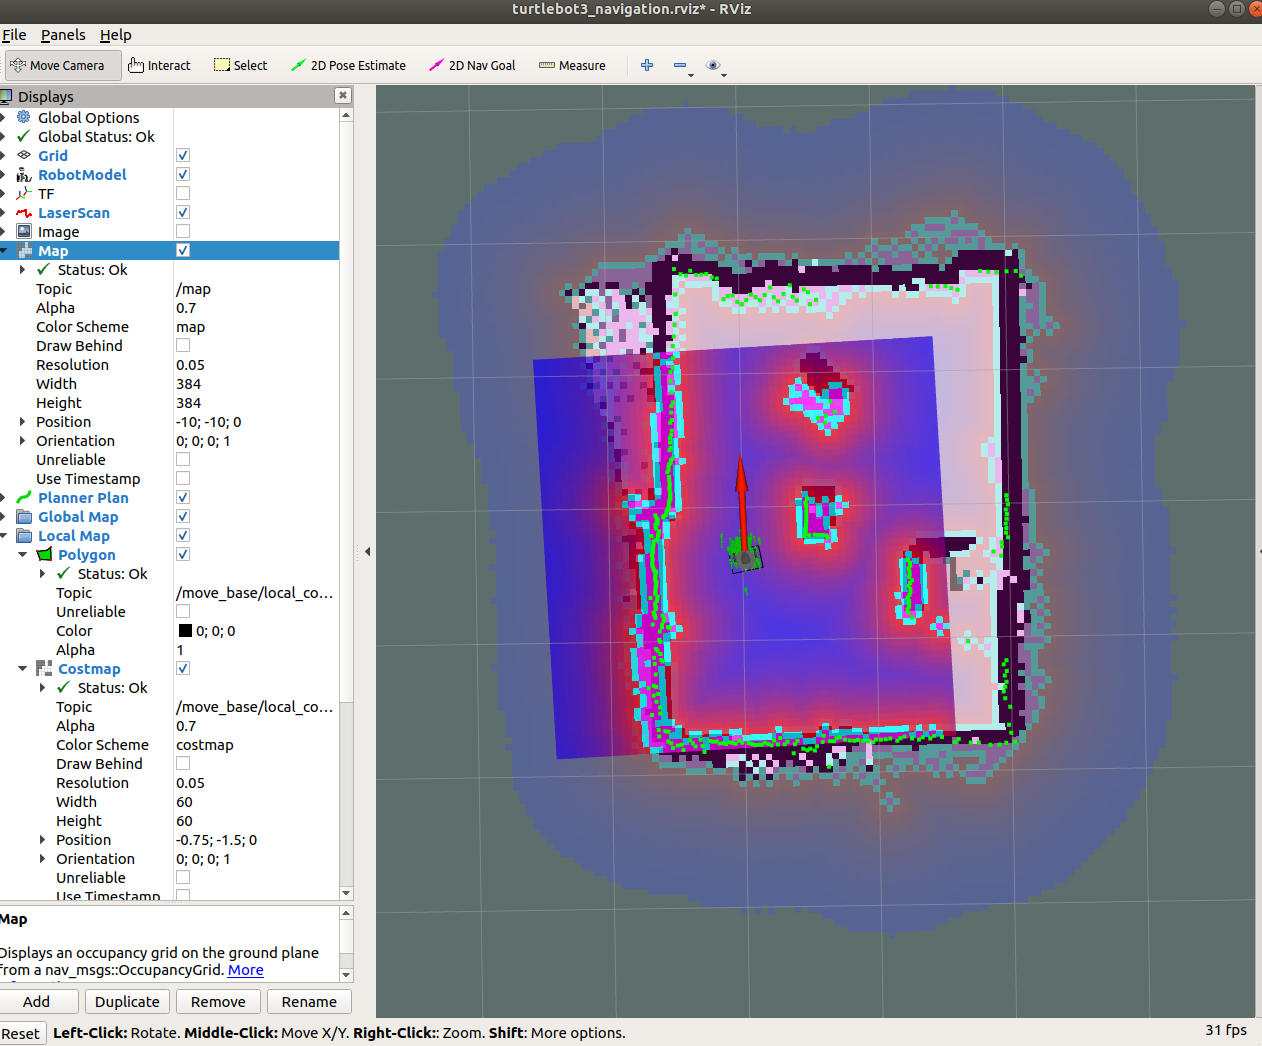
\includegraphics[width=1.0\linewidth]{figs/Rviz.png}
		\caption{Rviz}
		\label{Rviz}
	\end{center}
\end{figure}
%%%%画像とか入れたほうがいいでしょうか
%%%%入れたほうがいいです

実際に自律移動ロボットの研究を行う際は、PC上で表示している可視化した情報と現実空間を交互に見て比較を行う。
しかし、この作業を行いながらロボットの追跡を行うのは面倒であり、現実空間での位置関係はイメージしづらい。

比較を手助けする技術の1つにAR(Augmented Reality)技術があげられる。
ARとは、現実空間の映像にさまざまな情報を追加して表示する技術である。
自己位置推定の研究でもロボットが得た情報を現実空間に表示することで
交互に見るなどの作業を省くことで作業の効率化が見込められる。
また、比較の精度も可視化した情報が現実空間のどこに対応するのかイメージしながら行う従来の手法よりも高くなると考えられる。
ARを用いるメリットは、先行研究を踏まえて説明する。
%@@@これだけだとよくわからないので、あとで詳しく説明するとか書く。

\section{先行事例}

\subsection{AR ロボットコントローラ}
ARを用いた比較を容易にする技術の先行事例として、
鈴木による「ARロボットコントローラ」\cite{鈴木勇矢2019ARロボットコントローラ}がある。
「ARロボットコントローラー」とは、画面上のタップした地点にロボットを自律移動させることができるアプリケーションである。
また、ロボットの操作と同時にロボットの内部情報も表示することができる。
図\ref{ARロボットコントローラー}にアプリケーションを実行している際の様子を示す。
図\ref{ARロボットコントローラー}では以下の情報を表示している。
\begin{itemize}
      \item 赤い丸:ロボットの初期位置
      \item 青い丸:目的位置
      \item 黒い線:移動経路
      \item 黄色い点 :Lidarのデータ
      \item 緑色の矢印:自己位置推定の結果のパーティクル
   \item ロボットを囲う赤い円:ロボットの位置姿勢
\end{itemize}
このアプリケーションで標示するパーティクルとは、モンテカルロ位置推定(以下MCL)によって推定したパーティクルである。

\begin{figure}[H]
	\begin{center}
		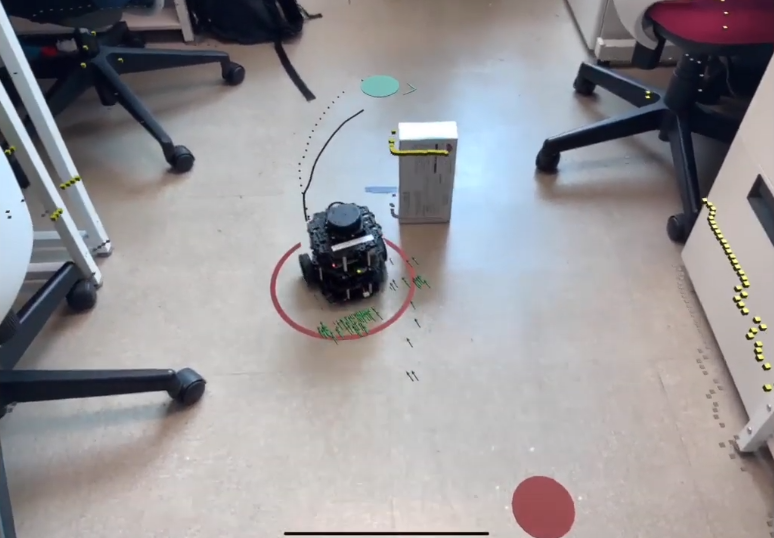
\includegraphics[width=1.0\linewidth]{figs/ARsuzuki.png}
		\caption{ARロボットコントローラー}
		\label{ARロボットコントローラー}
	\end{center}
\end{figure}
%画像

このアプリケーションのように、現実空間に内部情報を標示することで位置関係をイメージしやすくなる。
そのため、内部情報のデバックや評価もしやすくなると考えられる。

しかし、このアプリケーションの問題点として、一部の内部情報をアプリケーション上で正しく表示されないという問題点がある。
このアプリケーションでは、ロボットをオブジェクトとして認識し、ロボットがいる地点をパーティクルの中心と仮定してデータを表示している。
そのため、もしパーティクルがロボットから離れた位置を推定したとしても、パーティクルはロボットの周りに表示されてしまう。


\subsection{AR マーカーを用いた手法}
ARロボットコントローラの問題点を改善する手法として、高原によるARマーカーを用いる手法\cite{高原一樹2021ロボットの自己位置推定を可視化するAugmentedRealityアプリケーション}があげられる。
ARマーカーを用いる手法では、自己位置推定に用いるマップの原点にARマーカーを設置することで正しい位置に表示することを実現している。

しかし、ARマーカーを基準に表示を行うためARマーカーを見失ってしまうと表示しているデータの更新ができないという課題がある。
データの更新ができなくなる理由として、データを表示する際にARマーカーで座標を取得する必要があるためである。
そのため、ARマーカーを見失ってもアプリケーションを実行している端末が座標を推定する手段が必要だと考えられる。



% dvipdfmxとhereのテスト
%\begin{figure}[H]
%	\begin{center}
%		\includegraphics[width=1.0\linewidth]{../zero.png}
%		\caption{}
%		\label{fig:}
%	\end{center}
%\end{figure}
%
